\begin{figure*}[p]
	\centering
	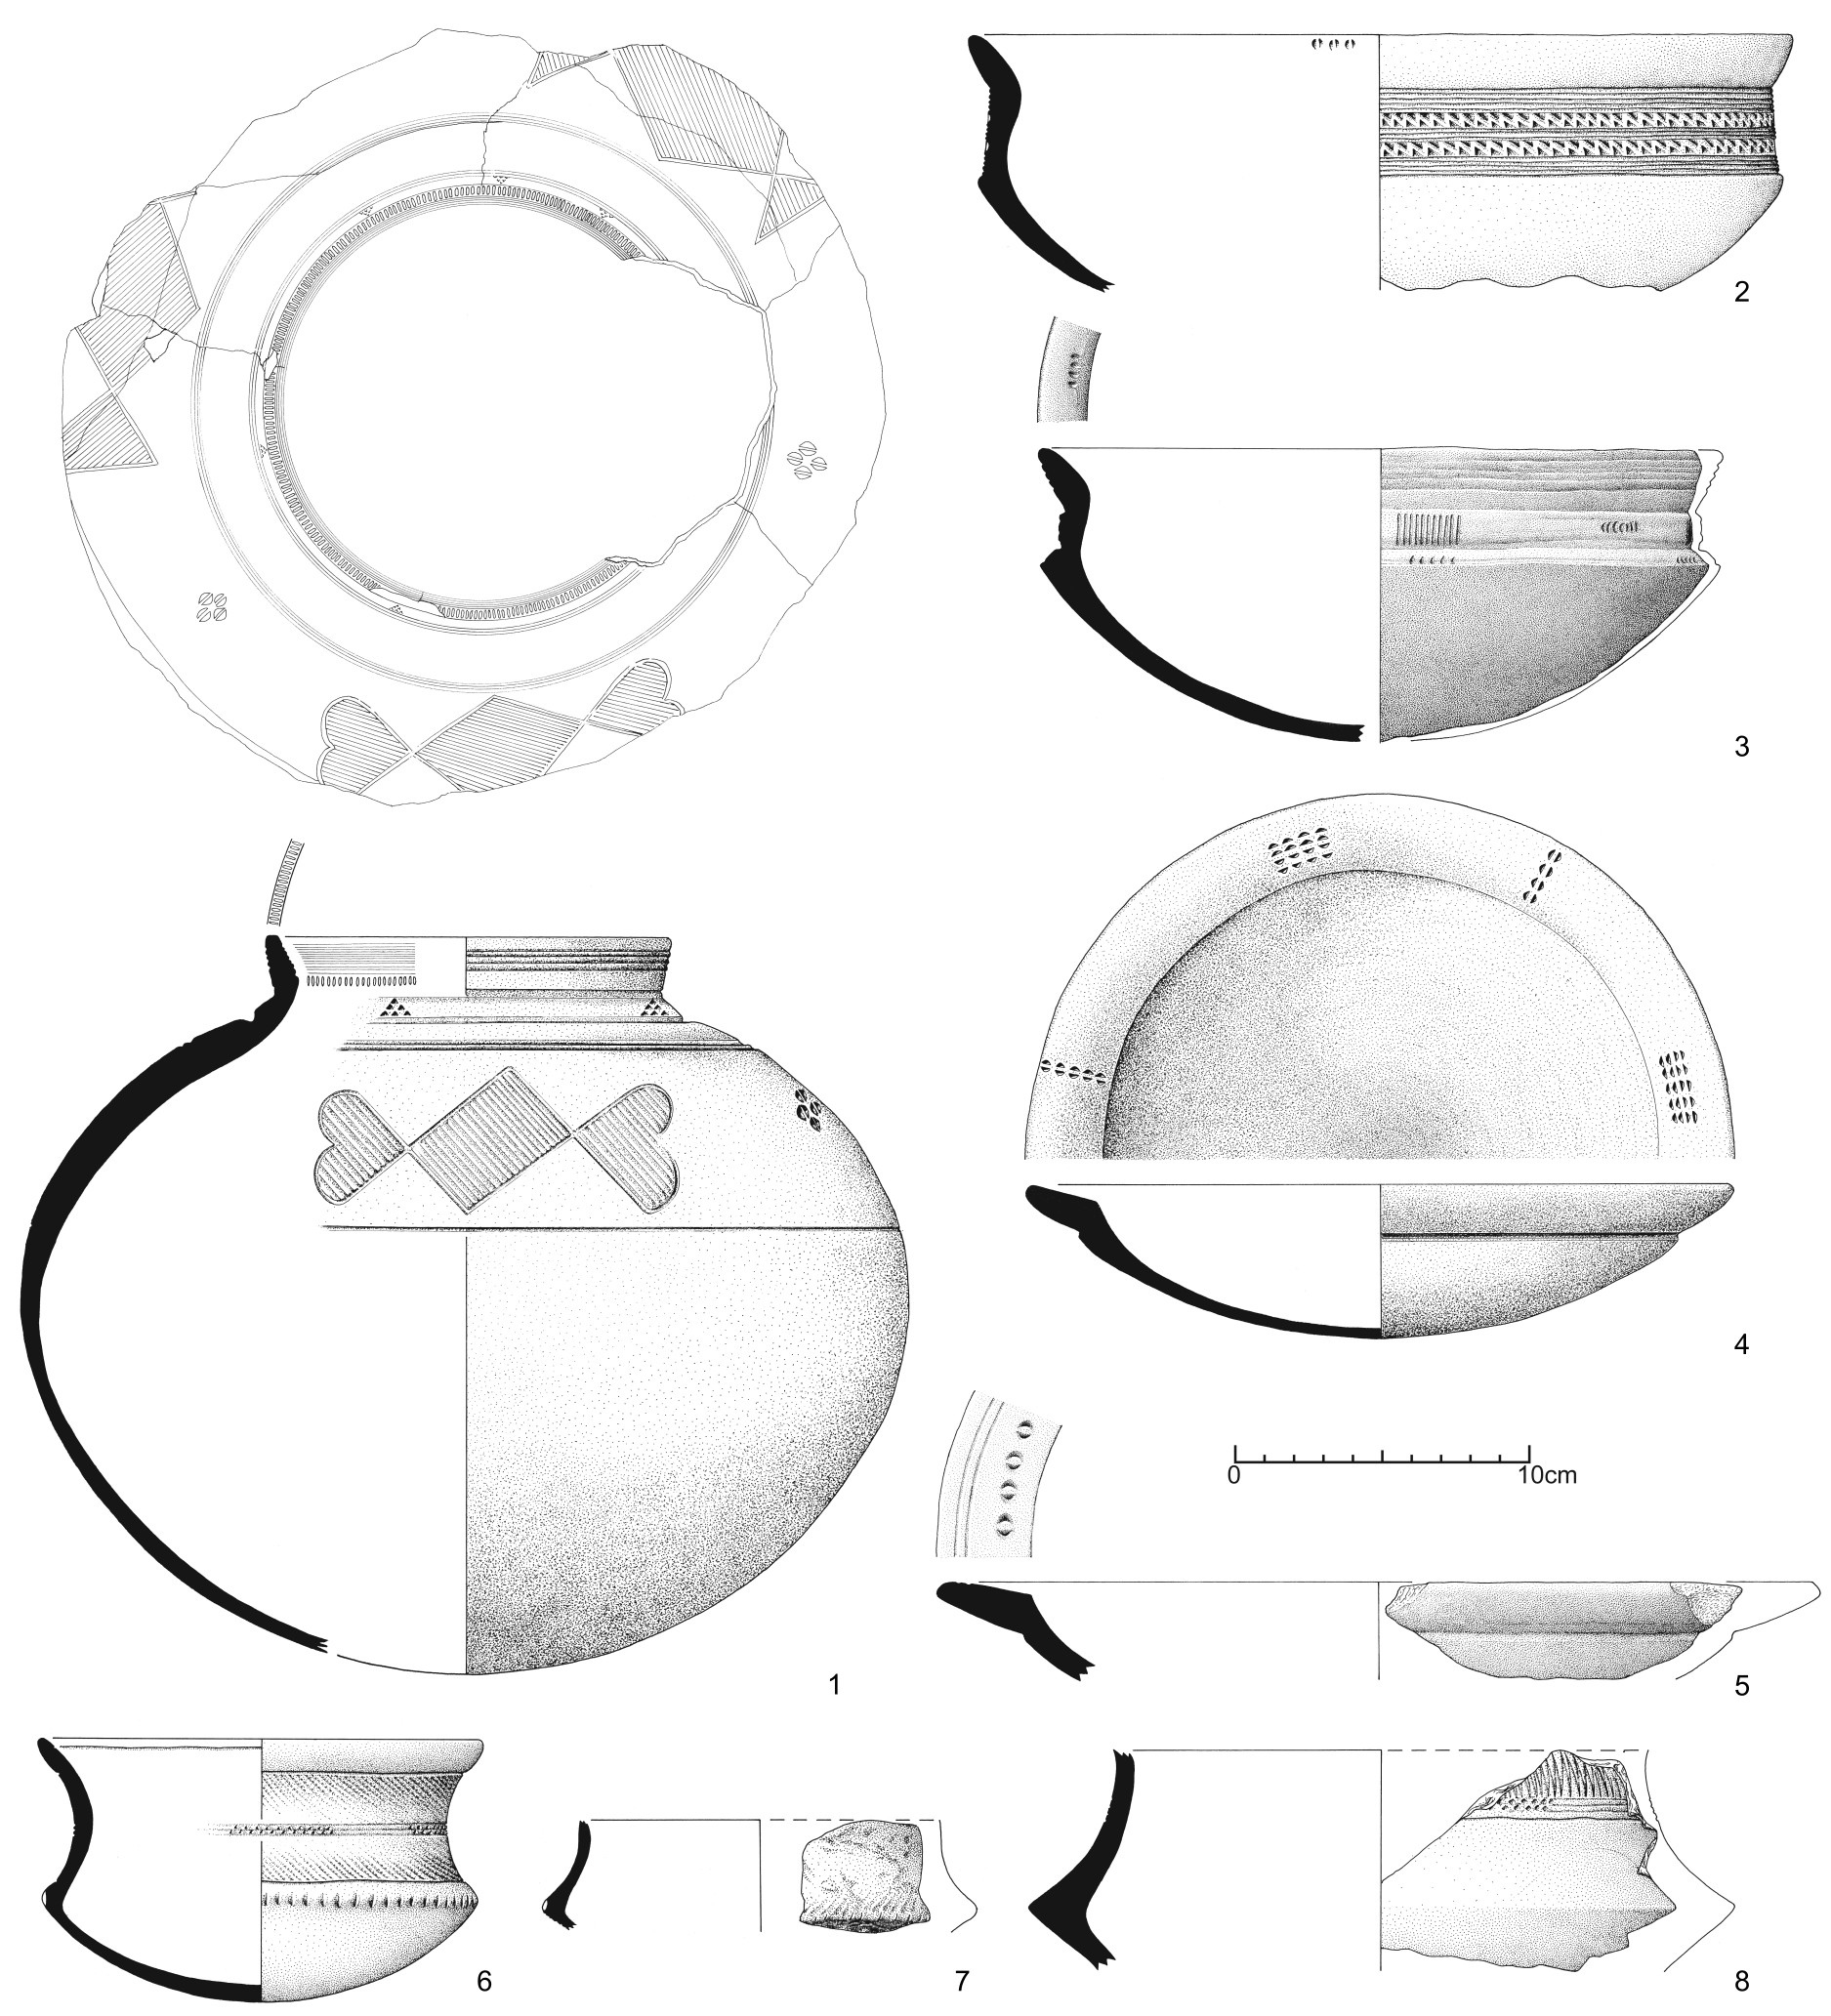
\includegraphics[width=\textwidth]{fig/NGO-Typen.pdf}
	\caption{Ngombe-Gruppe: Typvertreter aus Ngombe (Fpl.~252; Kat.-Nr.~11), Sosolo (Fpl.~241) und Bokonongo (Fpl.~250).\\1:~Taf.~43.1; 2:~Taf.~40.10; 3:~Taf.~42.15; 4:~44.1; 5:~Taf.~44.2; 6:~Taf.~42.16; 7:~Taf.~40.9; 8:~Taf.~36.13.}
	\label{fig:NGO_Typvertreter}
\end{figure*}

\begin{table*}[p]
	\centering
	{\footnotesize \begin{sftabular}{@{}lcccccc@{}}
			\toprule
			& \multicolumn{2}{c}{\textbf{Ngombe}} & \multicolumn{2}{c}{\textbf{\centering Longa}} & \multicolumn{2}{c}{\textbf{\centering Mbandaka}} \\
			& morph. & ornam. & morph. & ornam. & morph. & ornam. \\
			\midrule
			Große, bauchige Gefäße (G10a) & $\bullet$ & & & & $\circ$ & \\
			Knickwandschalen (G1a2/Typ 50) & $\bullet$ & & $\bullet$ & & & \\
			Teller (G12) & $\bullet$ & $\bullet$ & $\bullet$ & $\bullet$ & & \\ \hdashline[0.5pt/5pt]
			\textit{banfwa-nfwa}-Verzierung (V7) & \multicolumn{2}{c}{$\circ$}  & \multicolumn{2}{c}{$\bullet$} & \multicolumn{2}{c}{$\bullet$} \\
			Runde Böden (B1) & \multicolumn{2}{c}{$\bullet$} & \multicolumn{2}{c}{$\circ$} & & \\
			\bottomrule
	\end{sftabular}}
	\caption{Ngombe-Gruppe: Morphologische und ornamentale Übereinstimmungen zu den Stilgruppen Longa \parencite[121--128]{Wotzka.1995} und Mbandaka (ebd. 139--143).}
	\label{tab:NGO_Vgl_LON}
\end{table*}

\subsubsection{Ngombe-Gruppe}\label{sec:NGO-Gr}

Entlang des Unterlaufs des \mbox{Sangha} sowie dem \mbox{Likwala}-\mbox{aux}-\mbox{Herbes} und dem befahrenen Abschnitt des Kongo wurde eine Keramik erfasst, welche einerseits starke Ähnlichkeiten zu Stilgruppen des Inneren Kongobeckens, unter anderem den Gruppen Longa und Mbandaka, zeigt \parencite[121--128, 139--143]{Wotzka.1995}, andererseits aber auch deutlich eigenständige Charakteristika aufweist. Insgesamt wurden 56~GE von 15 verschiedenen Fundplätzen dieser nach der Fundstelle Ngombe am \mbox{Sangha} (Fpl. 252) benannten keramischen Stilgruppe zugerechnet. Die Hälfte aller aufgenommen Scherben der Ngombe-Gruppe sind Wandungsstücke. Zudem konnten sechs vollständige Gefäße dieser Stilgruppe zugewiesen werden. Der definierende Komplex für das Merkmalsspektrum der Ngombe-Gruppe ist die Keramikkonzentration NGO~87/102 (Kat.-Nr.~11) in Ngombe am \mbox{Sangha} (Fpl.~252; Abb.~\ref{fig:NGO_Typvertreter}).\footnote{Im Zuge der ursprünglichen Bearbeitung der Funde von 1987 fiel auf, dass aus dem Komplex NGO~87/101 aus Ngombe am \mbox{Sangha} (Fpl.~252), der das an der Oberfläche abgesammelte Material umfasst, keinerlei Funde vorliegen (\textsc{Eggert} 1990). Bei den Funden aus der an der Mündung des \mbox{Likwala}-\mbox{aux}-\mbox{Herbes} in den \mbox{Sangha} gelegenen Fundstelle Ngombe (Fpl.~283) fand sich neben dem Fundzettel für diesen Komplex noch ein weiterer Fundzettel, der mit NGO~87/101 beschriftet war. Es muss davon ausgegangen werden, dass die Funde der Komplexe NGO~87/101 aus Ngombe am \mbox{Sangha} und NGL~87/101 aus Ngombe am \mbox{Likwala}-\mbox{aux}-\mbox{Herbes} zu einem sehr frühen Zeitpunkt vermischt und beide Inventare anschließend mit der Kennung des letzten Komplexes (NGL~87/101) beschriftet wurden. Eine Vermischung der beiden Komplexe aus Ngombe selbst, des Materials von der Oberfläche (NGO~87/101) mit jenem aus der Keramikkonzentration (NGO~87/102, Kat.-Nr.~11) wurde bereits von den ersten Bearbeitern als wenig wahrscheinlich angesehen, da die Keramikkonzentration ein spezifisches Inventar weniger, aus einer Vielzahl von Fragmenten zusammensetzbarer Gefäße enthielt. Siehe Anm.~\ref{ftn:Vermischungen}.} Die daraus geborgene Keramik kann als zeitlich vergesellschaftet angesehen werden und entspricht sich in technischen wie formalen und ornamentalen Gesichtspunkten.

\paragraph{Technologische Merkmale}\hspace{-.5em}|\hspace{.5em}%
Die Scherben der Ngombe-Keramik enthalten praktisch keine nichtplastischen Partikel (89\,\%). Wenn Partikel in den Scherben beobachtbar sind, handelt es sich größtenteils um feinen Quarz. Bei 11\,\% der GE konnte ein Zusatz von zerstoßenen Keramikfragmenten im Scherben nachgewiesen werden. Ausschließlich Stücke von den beiden Fundplätzen Sosolo (Fpl.~241) und Monjolomba (Fpl.~243) am unteren \mbox{Sangha} ließen sich dem Schamott-gemagerten \textit{Fabric} 9 zuordnen (Tab.~\ref{tab:Fabrics_Bilder}). Keine Scherbe der Ngombe-Gruppe zeigt die Verwendung von rotbrennenden Tonen an. Etwa 70\,\% des Materials weist eine Färbung auf,  die eindeutig die Nutzung weißbrennender Tone anzeigt, während die Brennfarbe bei den restlichen Scherben nicht zweifelsfrei angesprochen werden konnte. Die GE der Ngombe-Gruppe zeigen durchweg geglättete Oberflächen, die in Einzelfällen auch leicht \textit{seifig} sein können. Lediglich etwa 10\,\% aller Stücke zeigen eine leicht raue Oberfläche. Die Wandungsdicke der Stücke lag im Mittel bei 6,9\,mm. 

\begin{figure*}[tb!]
	\begin{minipage}[b]{.66\textwidth}
		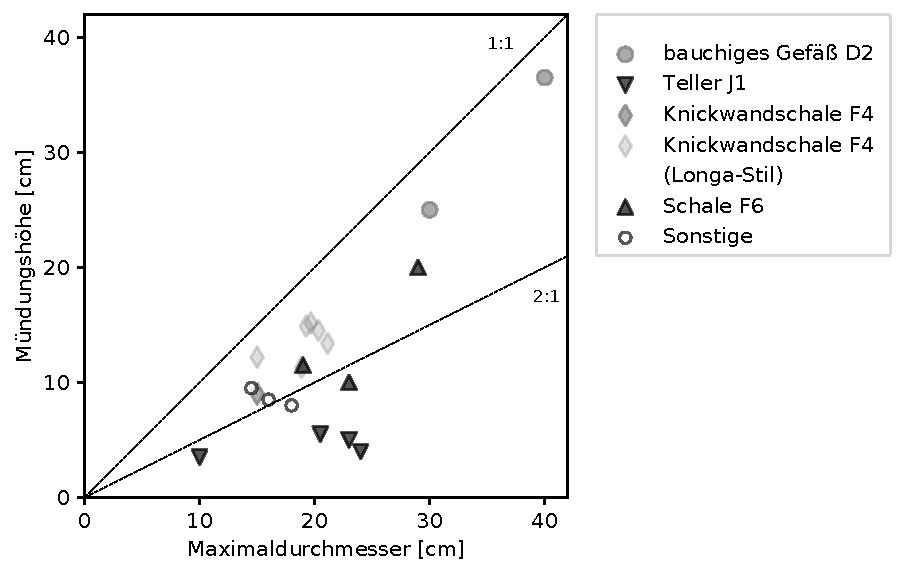
\includegraphics[width=\textwidth]{fig/NGO_Proportionen.pdf}
	\end{minipage}\hfill
	\begin{minipage}[b]{.33\textwidth}
		\caption{Ngombe-Gruppe: Proportionen (Knickwandschalen der Longa-Gruppe nach \textsc{Wotzka} 1995: 455 Taf.~21.2, 485 Taf.~51.9--10, 501 Taf.~67, 521 Taf.~87.4, 526 Taf.~92.6).\label{fig:NGO_Proportionen}}
	\end{minipage}
\end{figure*}

\paragraph{Formen}\hspace{-.5em}|\hspace{.5em}%
Bei 40 der insgesamt 56~GE der Ngombe-Gruppe konnte die Gefäßform bestimmt werden, allerdings war aufgrund von starker Fragmentierung bei 25\,\% eine sichere Ansprache nicht möglich. Den größten Anteil innerhalb der Keramik der Ngombe-Gruppe machen große Gefäße mit kurzem Kragen- oder nur leicht ausbiegendem Rand vom Typ D2 (40\,\%; Abb.~\ref{fig:NGO_Typvertreter}; Taf.~70.1) sowie Teller mit einem deutlichen Profilknick an der Innenseite aus (J1; 25\,\%; Abb.~\ref{fig:NGO_Typvertreter}.4--5).\footnote{Die Teller der Ngombe-Gruppe entsprechen morphologisch wie ornamental dem Typ~50 der Longa-Gruppe aus dem Inneren Kongobecken (\textsc{Wotzka} 1995: 121; Tab.~\ref{tab:NGO_Vgl_LON}).} Die großen, stark bauchigen Töpfe der Ngombe-Gruppe vom Typ D2 haben Durchmesser von bis zu 40\,cm, bei einer Höhe zwischen 25--36,5\,cm (Abb.~\ref{fig:NGO_Proportionen}). Die Teller des Typs J1 erreichen Durchmesser von bis zu 24\,cm und sind dabei zwischen 3,5--7\,cm hoch. Daneben umfasst das Formenspektrum auch kleine, flache Schalen mit Bauchabsatz und ausbiegendem Rand (Typ~E6; 10\,\%; Taf.~36.16--17, 38.15, 57.15) und flache Schalen mit scharfem Absatz im Bauchbereich und kurzem, ausbiegendem Rand (Typ~F6; 8\,\%; Abb.~\ref{fig:NGO_Typvertreter}.2--3). Etwas seltener finden sich flache Schalen mit starkem Bauchknick und deutlich ausgeprägtem, konkavem Halsbereich (Typ~F4; Abb.~\ref{fig:NGO_Typvertreter}.6--8)\footnote{Diese Form entspricht morphologisch den Knickwandschalen der Longa-Gruppe des Inneren Kongobeckens (Typ~44; \textsc{Wotzka} 1995: 121; 485~Taf.~14,9--10). Die Stücke der Ngombe-Gruppe des nordwestlichen Kongobeckens weisen jedoch eine andere Ornamentik als die Longa-Keramik auf.}, leicht bauchige Töpfe (Typ~C2) sowie Töpfe ohne ausgeprägten Halsbereich (Typ~E1). Das Gros der Ränder zeigt runde (M1; 42\,\%) sowie spitz (M2; 35\,\%) abgeschlossene Randlippen. In geringerem Maße fanden sich auch nach außen schräg abgestrichene Mündungsabschlüsse (M5, 12\,\%). Die am häufigsten angetroffene Randform innerhalb der Ngombe-Gruppe sind flach ausbiegende Ränder mit deutlichem Profilknick (B1.5; 32\,\%)\footnote{Die als B1.5 katalogisierte Randform entspricht den Typen R62 beziehungsweise R69 aus dem Inneren Kongobecken (\textsc{Wotzka} 1995: 122, 436 Taf.~2).}, welche den oben genannten Tellern des Typs J1 zuzuordnen sind. Die für die Ngombe-Gruppe charakteristischen großen, stark bauchigen Gefäße vom Typ D2 zeigen eine gewisse Heterogenität der Randgestaltung: durchweg kurze Varianten der Randformen A1, B1 sowie B2. Die zweithäufigste Randform innerhalb der Ngombe-Gruppe ist ein kurzer, leicht ausbiegender Rand (B1) an Schalen des Typs E6 und F6, die einen leicht konvexen Halsbereich sowie Absatz im Bauchbereich aufweisen. Bei 13~GE der Ngombe-Gruppe konnte die Form des Gefäßbodens bestimmt werden; in allen Fällen war der Boden rund ausgeformt (Typ~B1).

\paragraph{Verzierungen}\hspace{-.5em}|\hspace{.5em}%
Die Keramik der Ngombe-Gruppe ist grundsätzlich nur sporadisch verziert. Das mit Abstand am häufigsten angetroffene Verzierungselement sind horizontale Rillen (Tab.~\ref{tab:Verzierungselemente}: 02.1; 41\,\%). Diese finden sich durchweg auf der Innenseite und außen an den Rändern sowie im Hals- und Schulterbereich der Gefäße (Anlage~4\subref{fig:NGO_Verz}). Deutlich seltener und vor allem innen wie außen im Rand-, Schulter- und Bauchbereich finden sich horizontale Reihen aus einfachen Eindrücken (Tab.~\ref{tab:Verzierungselemente}: 04.15; 10\,\%). Eine Eigenheit der Ngombe-Keramik sind Gruppen aus kleinen, halbrunden Eindrücken beziehungsweise Einkerbungen, die fast ausschließlich an der Innenseite der Ränder zu finden sind (Tab.~\ref{tab:Verzierungselemente}: 04.5; 8\,\%). Des Weiteren umfasst das Spektrum an Verzierungselementen der Ngombe-Gruppe eine breite Palette von Ritz- oder Eindruckelementen (Tab.~\ref{tab:Verzierungselemente}: 01.1--3, 01.6, 01.8, 02.2--3, 02.5, 04.2--4, 04.8--9, 04.11--12, 04.17--18) sowie \textit{banfwa-nfwa}-Verzierungen (Tab.~\ref{tab:Verzierungselemente}: 08; 4\,\%) auf der Innenseite der Ränder sowie im Hals- und Schulterbereich (Anlage~4\subref{fig:NGO_Verz}). Die Ngombe-Gefäße zeigen eine klare Fokussierung der Verzierungen auf die Innenseite der Ränder sowie den Schulter- und Halsbereich. Insgesamt 75\,\% aller Verzierungen finden sich in diesen Abschnitten der Gefäße. Auf den Gefäßbäuchen finden sich nur sehr vereinzelt Verzierungen und die Gefäßunterteile sind bis auf Einzelfälle unverziert (\mbox{Anlage}~4\subref{fig:NGO_Verz}). Nur eine GE zeigt \textit{banfwa-nfwa} (Tab.~\ref{tab:Verzierungselemente}: 08) am Bodenansatz (Taf.~40.7).

\begin{figure*}[p]
	\centering
	\includegraphics[width=\textwidth]{fig/NGO_Verbreitung.pdf}
	\caption{Ngombe-Gruppe: Verbreitung.}
	\label{fig:NGO_Verbreitung}
\end{figure*}

\paragraph{Datierung}\hspace{-.5em}|\hspace{.5em}%
Für die Keramik der Ngombe-Gruppe liegen keine absoluten Daten vor. Der einzig potenziell datierbare Komplex, der für die Beschreibung der Gruppe bestimmenden Keramikkonzentration NGO~87/102 (Kat.-Nr.~11) in Ngombe am mittleren \mbox{Sangha} (Fpl.~252), konnte in den 1980er Jahren leider nicht direkt datiert werden.\footnote{Eine für eine Radiokohlenstoffdatierung vorgesehene Probe wurde nach Kiel eingeschickt, erbrachte aber nach der Aufbereitung keine ausreichenden Anteile organischen Materials. Nachforschungen ergaben leider kein weiteres datierbares Material aus diesem Komplex.} Mit Ausnahme dieses Komplexes stammt alles der Ngombe-Gruppe zugeordnete Fundmaterial von Oberflächenabsammlungen. Die Datierung der Ngombe-Keramik kann folglich lediglich anhand relativchronologischer Bezüge abgeleitet werden. Die der Ngombe-Gruppe zugeordnete Keramik weist deutliche Übereinstimmungen mit der Keramik der Longa-Gruppe des Inneren Kongobeckens sowie leichte Ähnlichkeiten zur Mbandaka-Gruppe auf (Tab.~\ref{tab:NGO_Vgl_LON}; \textsc{Wotzka} 1995: 121--128). Gerade die stark rundbauchigen Grundformen und abgesetzten Schulterpartien sowie die Fokussierung der Verzierung auf die Rand- und Schulterzonen erinnern an die Mbandaka-Gruppe des Inneren Kongobeckens (ebd. 139--143). Die Ngombe-Gruppe zeichnet sich, wie auch die Longa-Keramik (ebd. 123), durch runde Böden aus. Knickwandschalen des Typs F4 finden sich in beiden Stilgruppen. Jedoch weisen die GE der Longa-Gruppe (ebd. 455 Taf.~21.1--5, 456 Taf.~22.1--8, 475 Taf.~41.9, 485 Taf.~51.9--10, 503 Taf.~69.6--9, 507 Taf.~73.1--29) eine sehr viel elaboriertere Verzierung auf.

Die absolute Datierung der Longa-Gruppe ist gegenwärtig als unklar zu bezeichnen. Einerseits weist die Stilgruppe einen verbindenden Charakter zwischen den früheren Stilgruppen, vor allem Bokuma und Bokele, auf, andererseits stellt \textsc{Wotzka} (ebd. 127) fest, dass sie sich problemlos an das jüngere Ende der von ihm entwickelten Keramiksequenz anbinden lässt, welches vornehmlich durch die Bondongo-Gruppe charakterisiert ist. Die drei für die Longa-Gruppe vorliegenden Radiokohlenstoffdatierungen streuen vom 1.~Jt. v.~Chr. bis in das 12./13.~Jh. n.~Chr. (ebd. 127 Tab.~53).\footnote{Eine neuere Evaluation Wotzkas ergab eine höhere Wahrscheinlichkeit dafür, dass die jüngste der drei Datierungen, die in das 12./13.~Jh. n.~Chr. fällt (\textsc{Wotzka} 1995: 127 Tab.~53: Hv-11572), am ehesten repräsentativ für die chronologische Stellung der Stilgruppe ist. Siehe Kap.~\ref{sec:ICB_StilGrDatierungen}) und Anm.~\ref{ftn:fstafrikaWebStilGr-Tafeln}.}

Die Keramik der Mbandaka-Gruppe wird von Wotzka (ebd. 143) in eine zeitliche Nähe zur ins 11.--14.~Jh. n.~Chr. datierenden Bondongo-Keramik (ebd. 138 Tab.~58) gestellt, die wiederum starke Ähnlichkeiten zur Longa-Keramik aufweist. Für die Anbindung der Ngombe-Gruppe kann, bis eine direkte Datierung eines entsprechende Funde aufweisenden Komplexes vorliegt, nur eine den Stilen Longa und Mbandaka entsprechende, vom 12.--14.~Jh. n.~Chr. reichende Zeitstellung angenommen werden.

\paragraph{Verbreitung}\hspace{-.5em}|\hspace{.5em}%
Die Keramik der Ngombe-Gruppe wurde an insgesamt 15 verschiedenen Fundstellen im Bereich der Flussläufe des Kongo, \mbox{Sangha} sowie \mbox{Likwala}-\mbox{aux}-\mbox{Herbes} angetroffen. Das Verbreitungsgebiet besteht dabei aus zwei Kerngebieten; zum einen am mittleren \mbox{Sangha} zwischen Inyenge (Fpl.~249) und Ngombe (Fpl.~252) und zum anderen unmittelbar im Mündungsgebiet des \mbox{Sangha} in den Kongo (Abb.~\ref{fig:NGO_Verbreitung}). Die meisten Funde stammen aus dem letzteren Gebiet und hier vor allem von den beiden Plätzen Sosolo (Fpl.~241) und Monjolomba (Fpl.~243). Im Bereich nördlich, beziehungsweise flussauf von Ngombe (Fpl.~252), sowie am Kongo und \mbox{Likwala}-\mbox{aux}-\mbox{Herbes} fand sich ausschließlich Material, dessen Zuweisung zur Ngombe-Gruppe unter Vorbehalt erfolgte (Abb.~\ref{fig:NGO_Verbreitung}). Im Mündungsgebiet des Likwala-aux-Herbes, in Boleko (Fpl.~285), fanden sich lediglich zwei sicher der Ngombe-Gruppe zuweisbare GE.